\documentclass[border=10pt]{standalone}
\usepackage[svgnames]{xcolor}
\usepackage{amsmath}
\usepackage{pgfplots}
\pgfplotsset{compat=newest}
\usepackage[sfdefault]{FiraSans}
\usepackage{FiraMono}
\renewcommand*\familydefault{\sfdefault}
\begin{document}
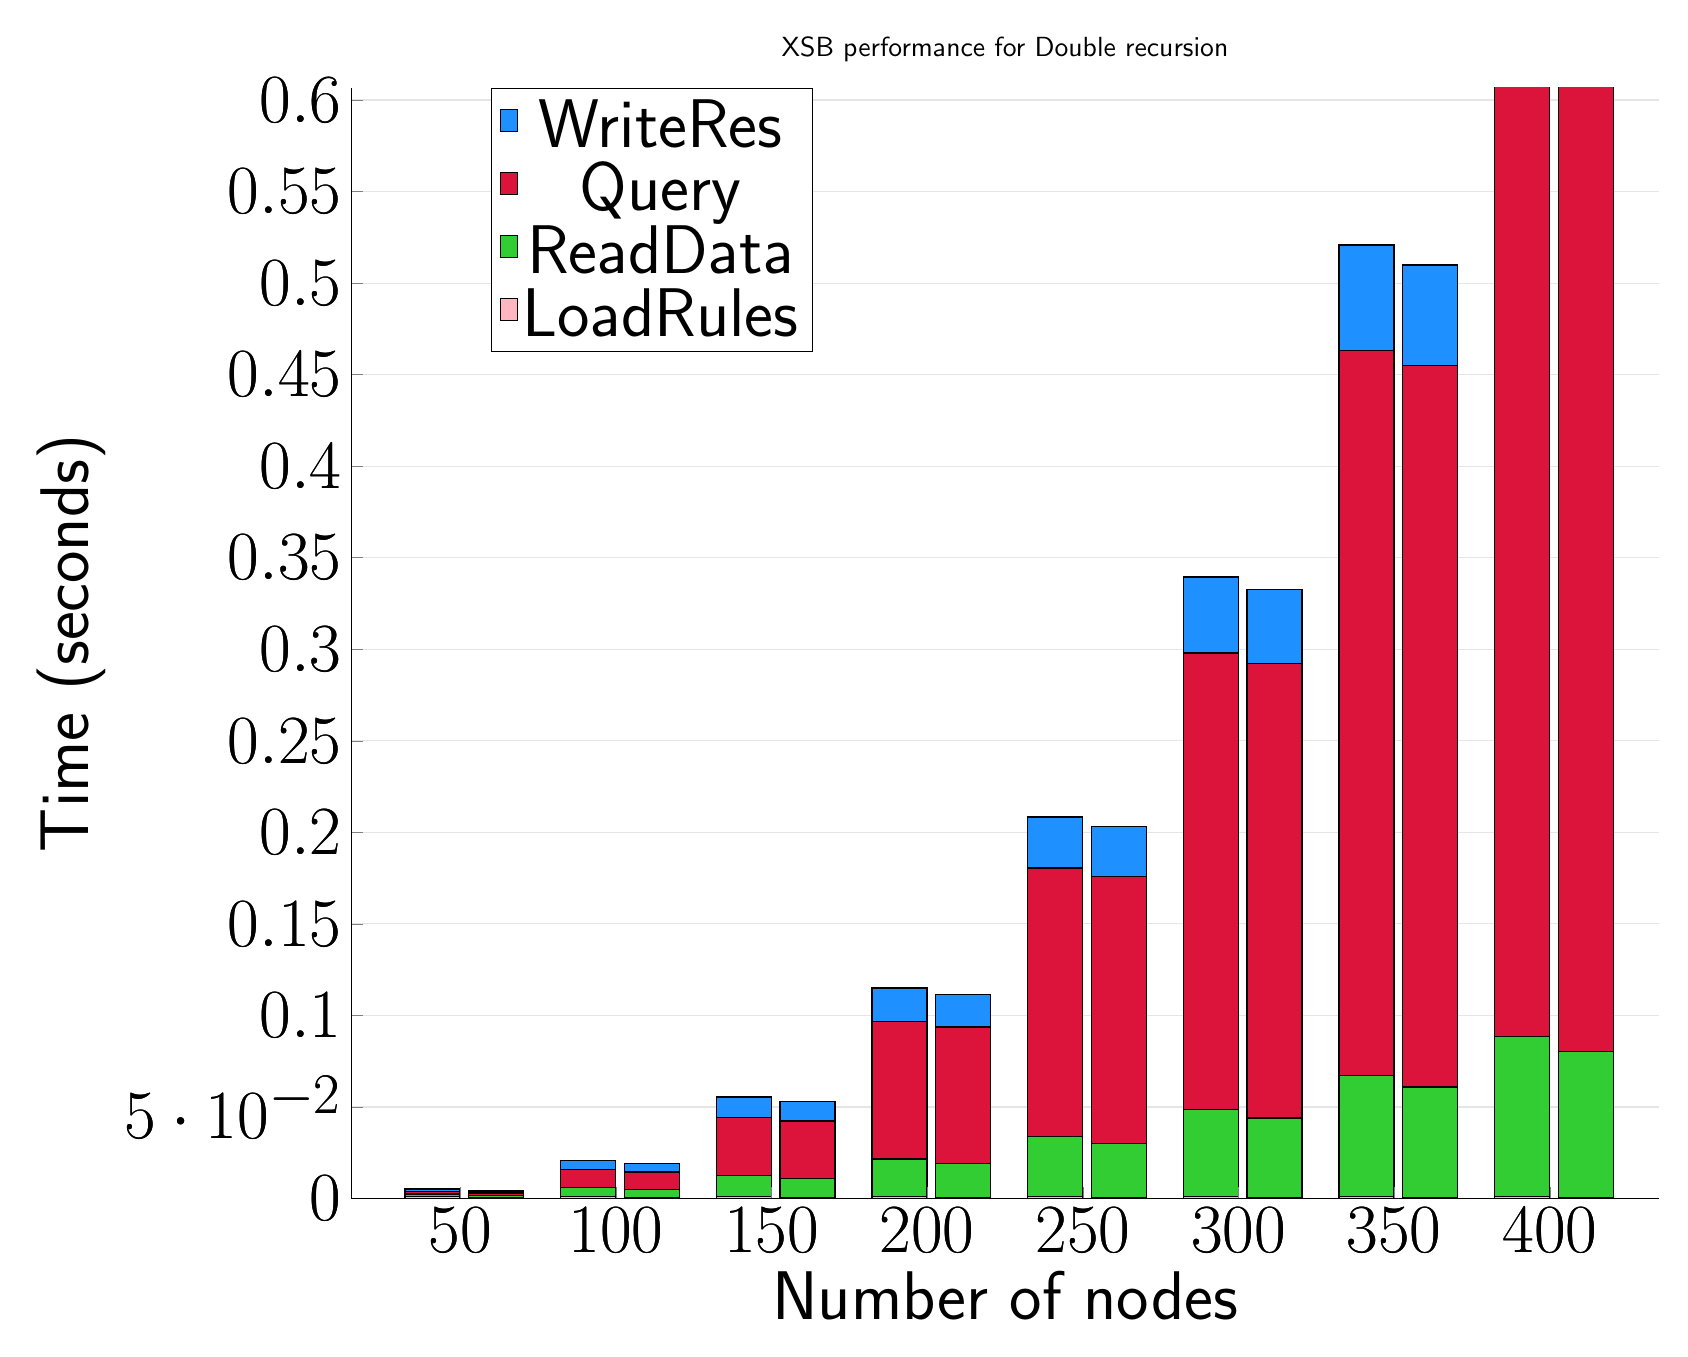
\begin{tikzpicture}
\begin{axis}[
   ybar stacked,
   title={XSB performance for Double recursion},
   bar shift=-10pt,
   width=1.5\textwidth,
   bar width=0.7cm,
   ymajorgrids, tick align=inside,
   major grid style={draw=gray!20},
   xtick=data,
   ymin=0, ymax=0.6066430044174194,
   axis x line*=bottom,
   axis y line*=left,
   enlarge x limits=0.1,
   legend style={
       at={(0.23, 1)},
       anchor=north,
       legend columns=1,
       font=\Huge,
   },
   ylabel={Time (seconds)},
   xlabel={Number of nodes},
   label style={font=\Huge},
   tick label style={font=\Huge},
]
\addlegendimage{fill=DodgerBlue, draw=black, line width=0.2pt}
\addlegendentry{WriteRes}
\addlegendimage{fill=Crimson, draw=black, line width=0.2pt}
\addlegendentry{Query}
\addlegendimage{fill=LimeGreen, draw=black, line width=0.2pt}
\addlegendentry{ReadData}
\addlegendimage{fill=LightPink, draw=black, line width=0.2pt}
\addlegendentry{LoadRules}
\addplot +[fill=LightPink, draw=black, line width=0.5pt] coordinates {
    (50, 0.001042580604553222)
    (100, 0.001053905487060546)
    (150, 0.001041793823242189)
    (200, 0.001057863235473632)
    (250, 0.001040053367614744)
    (300, 0.00107269287109375)
    (350, 0.0010960578918457029)
    (400, 0.0011265754699707029)
};
\addplot +[fill=LimeGreen, draw=black, line width=0.5pt] coordinates {
    (50, 0.0014657258987426749)
    (100, 0.005059933662414549)
    (150, 0.01142725944519045)
    (200, 0.020502662658691412)
    (250, 0.032857799530029305)
    (300, 0.04762797355651856)
    (350, 0.06598584651947023)
    (400, 0.08739480972290038)
};
\addplot +[fill=Crimson, draw=black, line width=0.5pt] coordinates {
    (50, 0.0013210773468017578)
    (100, 0.009639239311218262)
    (150, 0.03184030055999758)
    (200, 0.07507600784301757)
    (250, 0.1466784000396728)
    (300, 0.24935874938964847)
    (350, 0.3960703611373902)
    (400, 0.5866430044174193)
};
\addplot +[fill=DodgerBlue, draw=black, line width=0.5pt] coordinates {
    (50, 0.001323795318603515)
    (100, 0.004967784881591787)
    (150, 0.011213040351867678)
    (200, 0.018430995941162112)
    (250, 0.0277717113494875)
    (300, 0.0415011644363404)
    (350, 0.05771460533142071)
    (400, 0.0718007564544678)
};
\end{axis}
\begin{axis}[
   ybar stacked,
   bar shift=13pt,
   width=1.5\textwidth,
   bar width=0.7cm,
   ymajorgrids, tick align=inside,
   major grid style={draw=none},
   xtick=data,
   ymin=0, ymax=0.6066430044174194,
   axis x line*=none,
   axis y line*=none,
   enlarge x limits=0.1,
   label style={font=\Huge},
   tick label style={font=\Huge},
]
\addplot +[fill=LightPink, draw=black, line width=0.5pt] coordinates {
    (50, 0.0006057000000000001)
    (100, 0.0006084000000000003)
    (150, 0.0006120999999999998)
    (200, 0.0006119999999999999)
    (250, 0.0006014999999999998)
    (300, 0.0006125)
    (350, 0.0006228999999999998)
    (400, 0.0006317)
};
\addplot +[fill=LimeGreen, draw=black, line width=0.5pt] coordinates {
    (50, 0.0011666)
    (100, 0.0044178)
    (150, 0.010223)
    (200, 0.018557599999999997)
    (250, 0.029586499999999998)
    (300, 0.0433033)
    (350, 0.060255899999999994)
    (400, 0.079759)
};
\addplot +[fill=Crimson, draw=black, line width=0.5pt] coordinates {
    (50, 0.0013027)
    (100, 0.0095498)
    (150, 0.0315914)
    (200, 0.0746347)
    (250, 0.1458401)
    (300, 0.24822100000000002)
    (350, 0.3940025)
    (400, 0.5842841999999999)
};
\addplot +[fill=DodgerBlue, draw=black, line width=0.5pt] coordinates {
    (50, 0.0011030999999999999)
    (100, 0.0046101)
    (150, 0.010584199999999998)
    (200, 0.0177863)
    (250, 0.0273495)
    (300, 0.04059600000000001)
    (350, 0.05494140000000001)
    (400, 0.07059300000000002)
};
\end{axis}
\end{tikzpicture}

\end{document}
